\documentclass{article}
\usepackage[utf8]{inputenc}





\usepackage{caption}
%   \captionsetup{format=hang}
\usepackage{tikz} 
\usepackage{fancyhdr}
\pagestyle{fancy}
\usepackage{amsmath}
\usepackage{amsthm}
\usepackage{hyperref}
\usepackage[normalem]{ulem} 
\usepackage{authblk}
\usepackage{amsfonts}
\usepackage{tabularx}
\usepackage{mathrsfs}
\usepackage{csquotes}
\usepackage{amssymb}
\usepackage{titling}
\usepackage{relsize}
\usepackage{mathtools}
\DeclarePairedDelimiter\ceil{\lceil}{\rceil}
\DeclarePairedDelimiter\floor{\lfloor}{\rfloor}

\title{\Large 
An Exposition on Shor’s Factoring Algorithm and \\
Quantum Circuits for Modular Exponentiation
}

\author{ Daniel Hutama
        }
\date{\small Last updated: December 12, 2018}
        
\begin{document}

\maketitle

\begin{abstract}

This paper aims to provide an introductory, but thorough, study of Shor's quantum factoring algorithm. In contrast to typical high-level descriptions of the algorithm, we provide a detailed look at some quantum circuits for the modular exponentiation step in the period-finding subroutine. In particular, we highlight two distinctive circuit architectures for modular exponentiation to provide a comprehensive description of Shor's factoring algorithm. We assume readers have an understanding of basic number theory and quantum computing concepts, such as the Euclidean algorithm, qubits, and quantum logic gates.

\end{abstract}

\section{Introduction}\label{sec:introduction}

Integer factorization is a problem that has been studied by mathematicians for centuries, but has yet to see an efficient classical solution. The apparent intractability of the factorization problem has become the cornerstone of several cryptosystems, such as the widely used RSA encryption scheme \cite{RSA78}. 

In 1994, Peter Shor published a quantum algorithm capable of factoring an $n$-bit integer $N$ in a number of steps polynomial in the input size (i.e. the bit-length, $n$) \cite{Sho94}. A quantum computer running Shor's algorithm (with a sufficient number of qubits capable of maintaining quantum coherence) may one day make the large-$N$ factorization problem tractable. 

This paper seeks to provide a comprehensive description of Shor's algorithm, with a particular focus on the quantum circuit modules necessary to perform the computations. We first begin with a short primer on factoring via period finding. Following this, we present a high-level statement of the steps in Shor's period finding subroutine. In section \ref{sec:VedralSec}, we present a  classical-based reversible (unoptimized) quantum circuit developed by Vedral et. al. for implementing one of the subroutine's crucial steps. In section \ref{sec:BeauregardSec}, we discuss some circuit optimizations developed by Draper and Beauregard that reduce the total number of qubits needed to factor a given input. In the final section, we compare the two architectures and discuss their qubit requirements.

\section{Description of Shor's Algorithm}
\label{sec:ShorsDescription}
Instead of utilizing a brute-force approach to find the factors of $N$, Shor's algorithm considers a related number-theoretic problem. In particular, Shor's approach is to compute $r$, the period of $x$ modulo $N$, where $x$ is a randomly chosen seed value between $1$ and $N$. 

We proceed with a description of Shor's algorithm as shown in \cite{NC00}. Suppose we wish to factor a large semiprime number $N$. The factorization of $N$ can be accomplished via period-finding in five (high-level) steps (figure \ref{fig:flowchart}): 
\begin{enumerate}
\item Pick a random seed value $x$, with $1<x<N$.
\item Compute the greatest common divisor of $x$ and $N$. If $\gcd(x,N) \not= 1$, we have found a non-trivial factor of $N$. If $\gcd(x,N)=1$, continue to step 3.
\item Compute $r$, the period of $x \pmod{N}$, i.e. find $r$, such that $x^r \equiv 1 \pmod{N}$. This step is the focus of Shor's algorithm.
\item Check that $r$ is even and that $x^{r/2} \not \equiv \pm 1 \pmod{N}$. If either condition is violated, return to step 1. If neither are violated, continue to step 5.
\item The factorization of $N=pq$ is achieved by computing $p = \gcd(x^{r/2}+1, N)$ and $q = \gcd(x^{r/2}-1, N)$.
\end{enumerate}


\begin{figure}[!htbp]
\centering
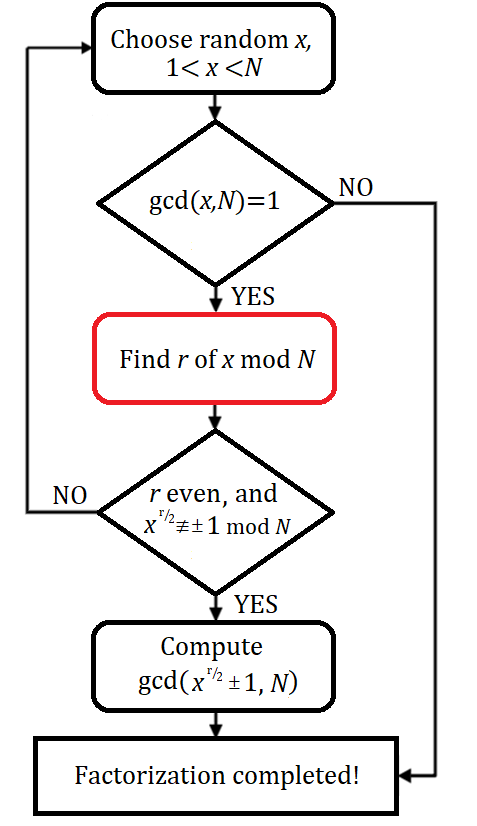
\includegraphics[width=.40\textwidth]
{flowchart.png}
\captionsetup{format = hang}
\caption{Flowchart of factoring via period-finding. The period-finding step is performed using a quantum computer running Shor's algorithm.}
\label{fig:flowchart}
\end{figure}
\pagebreak

We now proceed by describing the period finding step, which is made efficient on a quantum computer. Let Register 1 be a quantum register with $t\geq 2n$ qubits, where $n = \ceil*{\log_2(N)}$. Let Register 2 be a quantum register with $n$ qubits. Register 1 is used to hold the binary representation of integer states to be used as inputs to a quantum function. Register 2 is used to hold the $n$-bit outputs of the quantum function, which are entangled with the appropriate input states of Register 1. Shor's algorithm for period finding is as follows:
\begin{enumerate}
\item Initialize all quantum registers to the zero position. The state of the machine is denoted as $|0\rangle|0\rangle$, where the first ket corresponds to the state of Register 1, and the second ket corresponds to the state of Register 2.
\item Apply Hadamard gates to each of the $t$ qubits in Register 1. This performs the map $|0\rangle|0\rangle \to \dfrac{1}{\sqrt{2^t}}\mathlarger{\sum_{k=0}^{2^t-1}}|k\rangle|0\rangle$.
\item Apply a quantum function controlled by Register 1 on Register 2 that performs the map $\dfrac{1}{\sqrt{2^t}}\mathlarger{\sum_{k=0}^{2^t-1}}|k\rangle|0\rangle \to \dfrac{1}{\sqrt{2^t}}\mathlarger{\sum_{k=0}^{2^t-1}}|k\rangle|x^k \mod N\rangle$.
\item Apply a Quantum Fourier Transform to Register 1. This performs the map $\dfrac{1}{\sqrt{2^t}}\mathlarger{\sum_{k=0}^{2^t-1}}|k\rangle|x^k \mod N\rangle \to \dfrac{1}{{2^t}}\mathlarger{\sum_{k=0}^{2^t-1}\sum_{y=0}^{2^t-1}}\exp{\left(\dfrac{2\pi iky}{2^t}\right)}|y\rangle|x^k \mod N\rangle$.
\item Perform measurement of Register 1.
\item Use classical post-processing (continued fractions) to extract the period $r$ from the measurement performed in step 5.
\end{enumerate}


In summary, Shor's algorithm begins with a quantum computer whose registers are initialized to zero. The qubits in the first register are put in a superposition state using Hadamard gates. Following this, a function is applied on the second register, conditional on the states of qubits in the first register. A Fourier transform is applied to the first register to encode the function's period in a measurement probability amplitude. Finally, a measurement of the first register yields classical data, from which we can obtain the function's period using efficient classical methods.

\begin{figure}[!htbp]
\centering
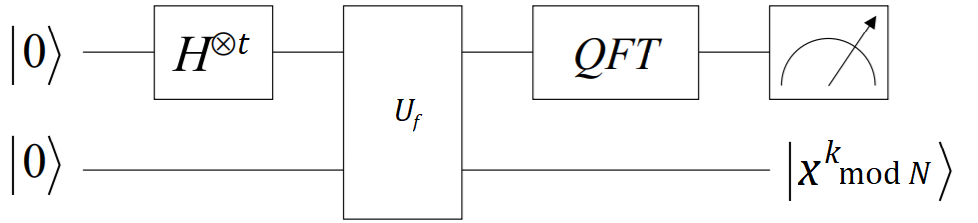
\includegraphics[width=.80\textwidth]
{shorshighlevel.png}
\captionsetup{format = hang}
\caption{High-level circuit depiction of Shor's algorithm. A description of the QFT module can be found in \cite{Dra00}.}
\label{fig:shorscircuit}
\end{figure}

\pagebreak

\section{Classical-based circuit}
\label{sec:VedralSec}


\begin{figure}[!htbp]
\centering
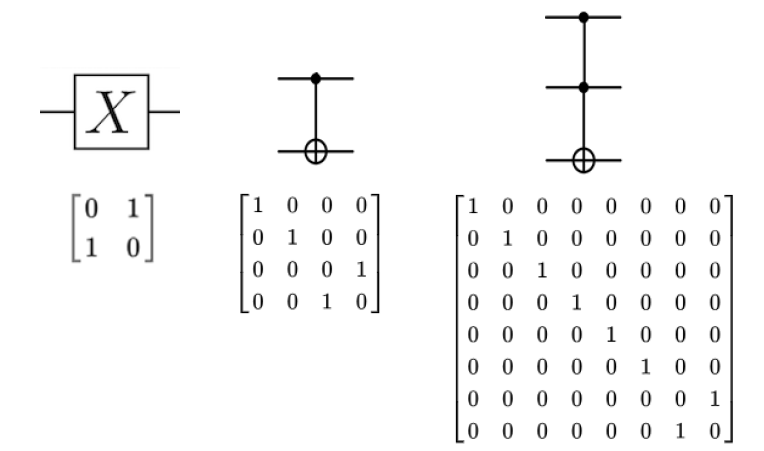
\includegraphics[width=.7\textwidth]
{vedralgateset.png}
\captionsetup{format = hang}
\caption{Gate set used in Vedral's quantum modular exponentiation circuit. From left to right: X gate, controlled-NOT gate, and Toffoli Gate.}
\label{fig:vedralgates}
\end{figure}
From the gates shown in figure \ref{fig:vedralgates}, we show how Vedral constructs a network for quantum modular exponentiation. We start by describing a circuit to perform the addition of two quantum registers. We then show how several plain addition circuits can be networked to create a modular addition circuit. Before continuing to the modules that utilize entanglement between Register 1 and Register 2, we present a mathematical description of the controlled modular multiplication and exponentiation gates. We note that Dirac kets on quantum register states in some figures have been dropped for consistency with Vedral's notation. All register states in this section should be considered as quantum.
\begin{figure}[!htbp]
\centering
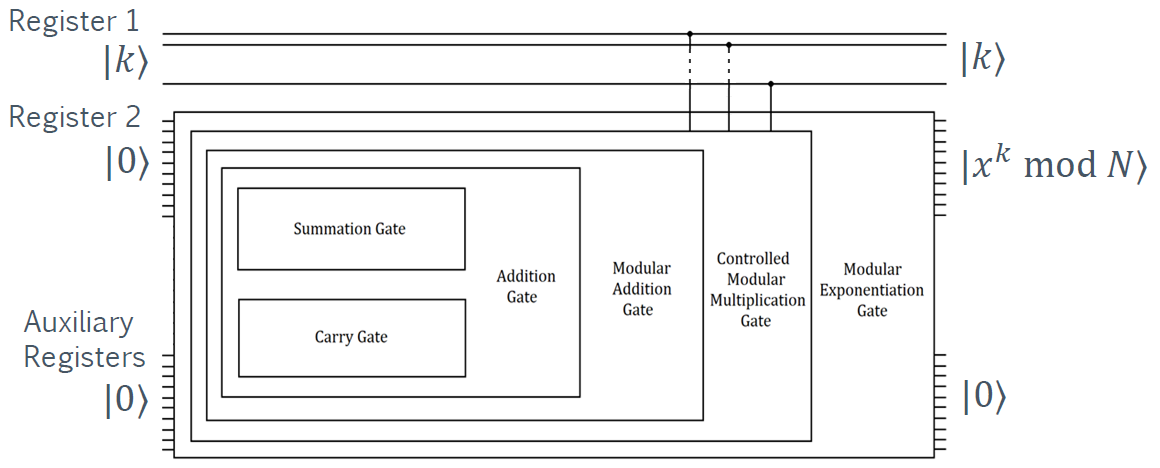
\includegraphics[width=1\textwidth]
{levelscheme.png}
\captionsetup{format = hang}
\caption{L.}
\label{fig:levelscheme}
\end{figure}


\subsection{Quantum ADDER gate}
\label{sec:vedralADDER}
The first main building block in Vedral's modular exponentiation circuit is the plain ADDER gate (figure \ref{fig:vedralADDER}). The quantum plain ADDER gate is constructed using and array of smaller SUM and CARRY gates, which are composed of CNOT and Toffoli gates (figure \ref{fig:carrysumgates}).
\begin{figure}[!htbp]
\centering
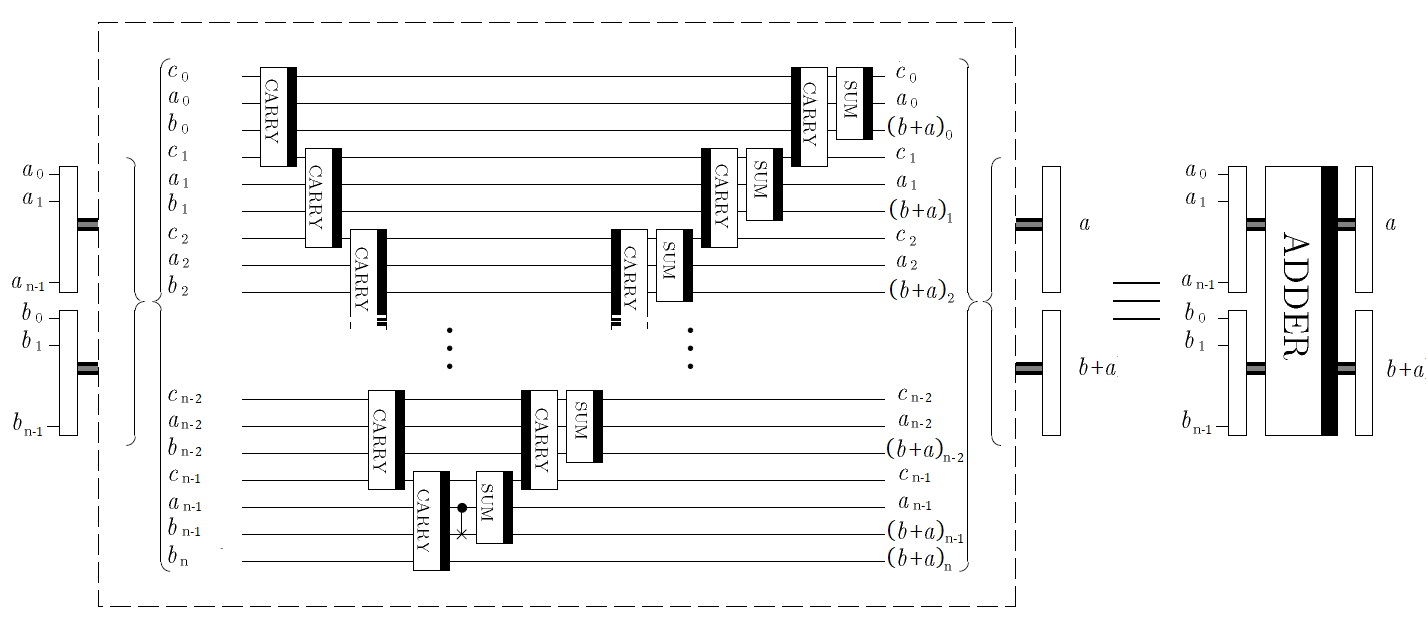
\includegraphics[width=1\textwidth]
{vedraladder.png}
\captionsetup{format = hang}
\caption{Vedral's Quantum ADDER gate from \cite{VBE95}.}
\label{fig:vedralADDER}
\end{figure}

\begin{figure}[!htbp]
\centering
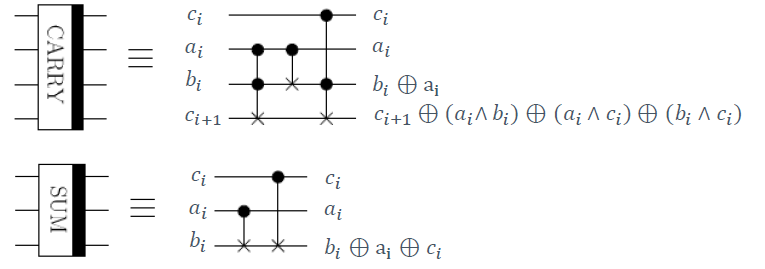
\includegraphics[width=.8\textwidth]
{carrysumgates.png}
\captionsetup{format = hang}
\caption{CARRY (top) and SUM (bottom) gates used in the classical-based reversible quantum ADDER gate design. Thick black bars are used to denote the forward operation of the quantum gate.}
\label{fig:carrysumgates}
\end{figure}

The quantum plain ADDER gate's goal is to take its input registers $|a\rangle |b\rangle$ to the state $|a\rangle |b+a\rangle$. The first $n$ CARRY gates in figure \ref{fig:vedralADDER} compute the most significant bit (MSB) of $b+a$ in the gate's lower register. The value of the MSB is then stored in $b_n$, which is the MSB of $b$. In order to accomplish this, we require an auxiliary ``carry register'' of size $n$ (which can be reduced to $n-1$ by observing $c_0$ remains unchanged from 0) to store the output of each CARRY gate. Following the final forward CARRY gate, a CNOT is used to reverse the action of the final carry on $b_{n-1}$. The subsequent array of reversed CARRY gates and forward SUM gates computes the value of $|b+a\rangle$ in the second input register, while also unitarily resetting the auxiliary register to the zero state. 



\subsection{Quantum ADDER MOD gate}
\label{sec:vedralADDERMOD}
Modular addition is accomplished using a fixed-length series of quantum ADDER gates. In particular, we require five ($5$) total quantum ADDER gates to accomplish modular addition. 

\begin{figure}[!htbp]
\centering
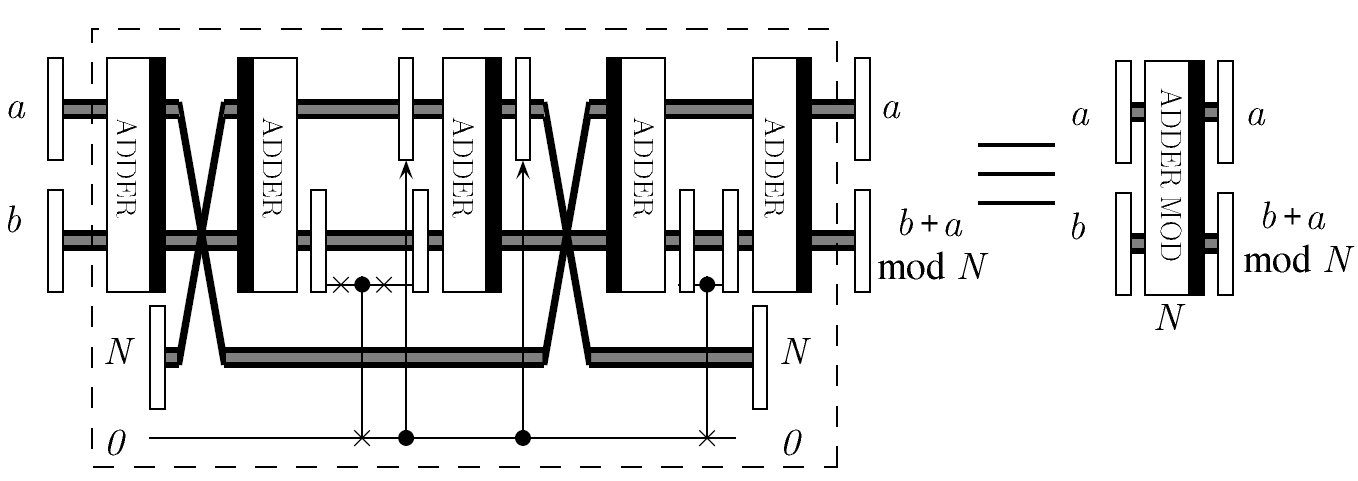
\includegraphics[width=1\textwidth]
{vedraladdermod.png}
\captionsetup{format = hang}
\caption{Vedral's Quantum ADDER MOD N gate. Adapted from \cite{VBE95}.}
\label{fig:vedralADDERMOD}
\end{figure}

The effect of the first ADDER gate in figure \ref{fig:vedralADDERMOD} is to perform the mapping $|a\rangle |b\rangle$ to $|a\rangle |b+a\rangle$, where the lower register outputs the summation of the input registers. Following this, the integer to be factorized, $N$, is loaded into the upper register of the subsequent reversed ADDER gate. The inputs to the second gate are then $|N\rangle |b+a\rangle$. The output of the second ADDER gate depends on the value of $N$ relative to $b+a$. If $N<b+a$, the output of the second gate will be simply $|N\rangle|(b+a)-N\rangle$, where the lower register outputs a simple subtraction. However, if $N>b+a$, the lower register outputs the complementary state $|2^{n+1} - [N - (b+a)]\rangle$.  

In the case when $N > b+a$, we wish to add back $N$ so that the final output is properly $b+a \mod N$. On the other hand when $N<b+a$, we wish to add the value 0, such that the final output is $b+a - N$ to give the proper value modulo $N$. This can be accomplished by using the MSB of the answer register as a control qubit. This qubit conditionally determines whether the register containing $N$ is set to the zero state prior to the third ADDER gate. After the third ADDER, the register containing $N$ is (conditionally) restored to its input. The final two ADDER gates unitarily reset the auxiliary qubits to allow the overall ADDER MOD circuit to be used as a module in the next component. 

\vspace{1em}
\noindent\large{\textbf{Strategy for implementing modular exponentiation}}
\vspace{.5em}

\normalsize 
	Before continuing with the (controlled) modular multiplication gate, we first discuss some general strategy to construct a circuit that performs $|k\rangle|0\rangle \to |k\rangle|x^k \mod N\rangle$. 
    
    Let $f(k) = x^N \mod N$ denote the function we wish to implement, where $k$ is the integer encoded in Register 1, $x$ is the randomly chosen seed value, and $N$ is the number we wish to factorize. Let $t \geq 2n$, where $n = \ceil*{\log_2(N)}$, be the size of Register 2. We can decompose $f(k)$ into a series of $t$ multiplications using properties of the binary representation of $k$. For $k = 2^0k_0 +2^1k_1 + \ldots + 2^{t-1}k_{t-1}$, we can rewire $f(k)$ as
    \begin{align}
    f(k) &= x^{2^0k_0 +2^1k_1 + \ldots + 2^{t-1}k_{t-1}} \mod N \nonumber \\ 
    &= \left(...\left(\left((x^{2^0k_0}) \text{ mod }N \cdot x^{2^1k_1} \right) \text{mod } N	\right)\cdot ... \cdot x^{2^{t-1}k_{t-1}}\right) \text{mod } N \nonumber \\
    &= \prod_{j=1}^{t-1} x^{2^j k_j} \text{ mod } N \text{  } | \text{  } \text{mod } N,
    \label{eq:modexp}
    \end{align}
where we have used a distributive property of the modulo operation to write $f(k)$ as $t$ repeated multiplications with evaluation modulo $N$ after each multiplication in equation \eqref{eq:modexp}.

Now that we have shown that modular exponentiation can be constructed with $t$ repeated modular multiplications, we now proceed by showing that modular multiplication can be accomplished with $n$ repeated modular additions. In particular, we wish to show how to construct a module that takes some input $\gamma \to (\gamma x^{2^j k_j}) \text{ mod } N$ using the state of qubits in Register 1 as control qubits. Note that any $x^{2^j k_j}$ term in equation \eqref{eq:modexp} can be decomposed into $n$ additions using the properties of its binary representation:
\begin{equation*}
\left(2^0(x^{2^j})_0 + 2^1(x^{2^j})_1 + ... + 2^{t-1}(x^{2^j})_{t-1}\right)^{k_j} = \left(\sum_{i=0}^{t-1}2^i(x^{2^j})_i\right)^{k_j},
\end{equation*}
which will be 1 if $k_j=0$. Thus, for some input $\gamma$ to our $k_j$-controlled multiplication gate, we wish to output
\begin{equation}
\label{eq:ctrlmult}
\gamma x^{2^j k_j} \text{ mod } N = 
\begin{cases}
    \mathlarger\sum_{m=1}^{n-1}2^m\gamma_mx^{2^j} \text{ mod } N \text{  } | \text{  } \text{mod } N, & \text{if } k_j =  1\\
    \gamma ,       & \text{if } k_j = 0,
\end{cases}
\end{equation}
where $\gamma$ in equation \eqref{eq:ctrlmult} will be the output from the previous controlled multiplication gate. In summary, we require our controlled modular multiplication gate to perform $n$ repeated modular additions with evaluation mod $N$ when $k_j = 1$, and to conditionally load $2^m x^{2^j} \text{ mod } N$ in the upper register of the appropriate ADDER MOD component if $k_j \wedge \gamma_m = 1$.

\subsection{Quantum Ctrl-MULT MOD gate}
\label{sec:vedralCTRLMULTMOD}
Modular multiplication is accomplished using a series of $n$ doubly controlled ADDER MOD N gates. Each Ctrl-MULT MOD gate takes some input $\gamma$, which will be the output from the preceding Ctrl-MULT MOD gate, and maps it to $\gamma x^{2^j} \text{ mod }N$.
\pagebreak
\begin{figure}[!htbp]
\centering
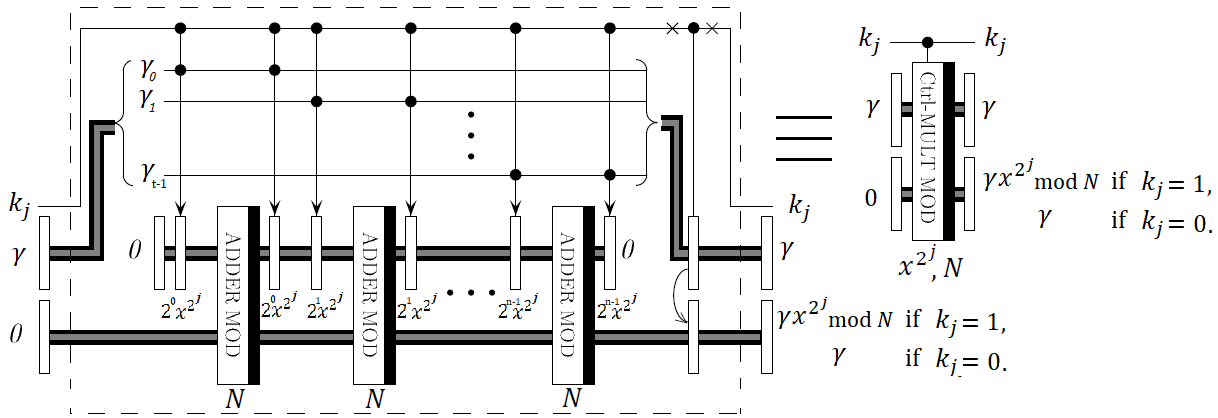
\includegraphics[width=1\textwidth]
{vedralcrtlmultmod.png}
\captionsetup{format = hang}
\caption{Vedral's Quantum Ctrl-MULT MOD gate. Adapted from \cite{VBE95}. The classically computed values (conditionally) loaded on the auxiliary register are loaded modulo $N$.}
\label{fig:vedralCTRLMULTMOD}
\end{figure}

In figure \ref{fig:vedralCTRLMULTMOD}, the upper register of the series of ADDER MOD N gates is an auxiliary register, which is conditionally loaded with the classically computed value of $2^m x^{2^j} \text{ mod } N$. After the action of each gate, the auxiliary register is immediately unloaded and conditionally reloaded with the next value. In the case when $k_j = 0$, the input value, $\gamma$, is copied to the output of the lower (answer) register for use in the next Ctrl-MULT MOD gate.

For example, suppose $k_j = 1$. The upper (auxiliary) register is loaded with the classically computed value $2^0\gamma_0x^{2^j} \text{ mod }N$. The output on the lower (answer) register is $(0 + 2^0\gamma_0x^{2^j} \text{ mod }N) \text{ mod } N$. Following the action of the first ADDER MOD N gate, the auxiliary register is unloaded to zero and reloaded with the classically computed value of $2^1\gamma_1x^{2^j} \text{ mod }N$. After the action of the second ADDER MOD N gate, the lower register contains a value of $\left((0 + 2^0\gamma_0x^{2^j} \text{ mod }N) \text{ mod } N + 2^1\gamma_1x^{2^j} \text{ mod } N\right) \text{ mod }N$. This process occurs a total of $n$ times to produce an output of 
\begin{equation*}
\sum_{m=0}^{n-1}2^m \gamma_m x^{2^j} \text {  }|\text{  mod }N = \gamma x^{2^j} \text{ mod } N,
\end{equation*}
which is what we showed in equation \eqref{eq:ctrlmult} for $k_j = 1$.


\subsection{Quantum Modular Exponentiation}
Modular exponentiation is accomplished using a series of $2t$ Ctrl-MULT MOD gates, where $t\geq 2n$. The overall circuit implements the $U_f$ function shown in figure \ref{fig:levelscheme}.
\pagebreak
\begin{figure}[!htbp]
\centering
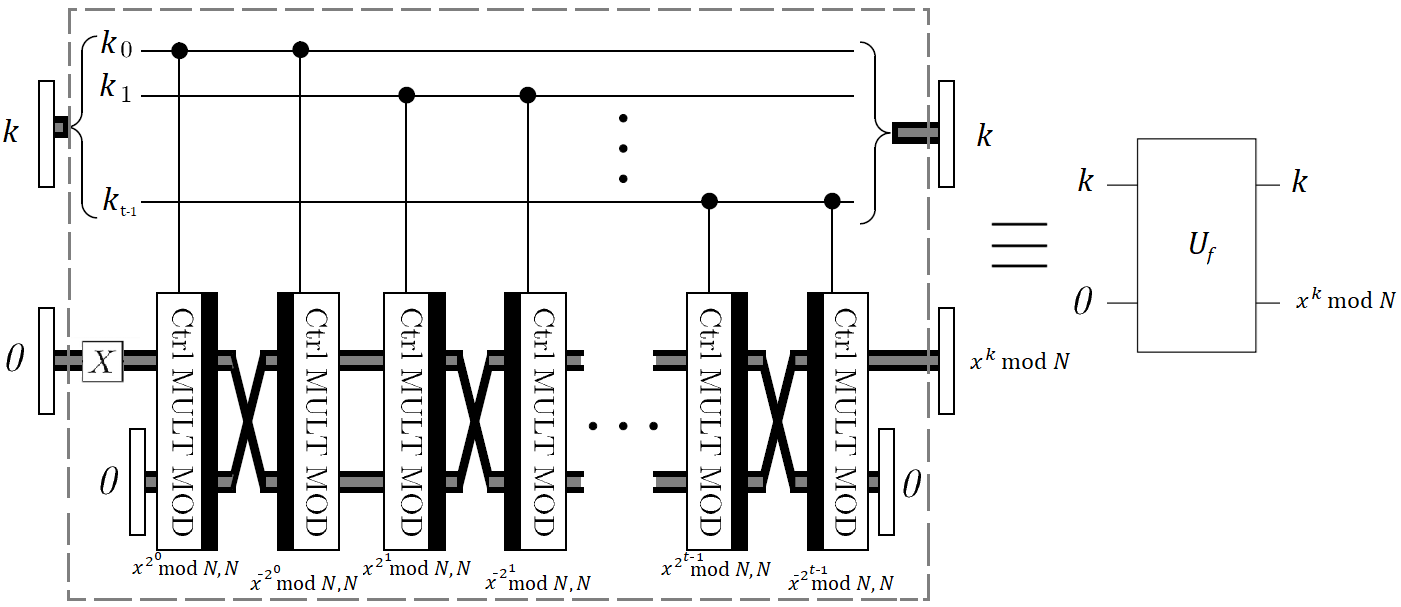
\includegraphics[width=1\textwidth]
{vedralexpmod.png}
\captionsetup{format = hang}
\caption{Vedral's Quantum modular exponentiation gate. Adapted from \cite{VBE95}.}
\label{fig:vedralexpmod}
\end{figure}

Register 2, which is the lower input register in figure \ref{fig:vedralexpmod}, is initially in the zero state. The single Pauli X gate prior to the first Ctrl-MULT MOD gate in the circuit acts on the LSB of Register 2. This encodes the value of 1 in the input to ensure that the output of the first Ctrl-MULT MOD gate is either $x^{2^0} \text{ mod }N$ or $1$, conditional on the value of $k_0$. Following the action of the first gate, the upper and lower registers are swapped. The subsequent Ctrl-MULT MOD gate is run in reverse and has its registers loaded with the classically computed value of $x^{-2^0} \text{ mod }N$. The effect of implementing the modular multiplicative inverse is to set the lower input register of the third Ctrl-MULT MOD gate to the zero state, while preserving the output of the first gate in the upper register \cite{VBE95}. This process is repeated $t$ times (once for each $k_j$ for $j\in [0, t-1]$) until the output contains the desired $f(k) = x^k \text{ mod } N$ function. More precisely, the sequence of Ctrl-MULT MOD gates implements 
\begin{equation*}
\prod_{j=0}^{t-1} x^{2^j k_j} \text{ mod }N \text{  } | \text{  mod }N,
\end{equation*}
which we showed to be equal to $f(k) = x^k \text{ mod }N$ in equation \eqref{eq:modexp}.


\section{Fourier space circuit}
\label{sec:BeauregardSec}
In this section, we present improvements to the classical-based design of Vedral et al. by T. Draper \cite{Dra00} and S. Beauregard \cite{Bea03}. Draper's circuit for quantum addition eliminates the need for an auxiliary carry register, while Beauregard's circuits extend some of Draper's methodology to other modules for further optimizations. After the presentation of the improved circuits, we analyze the qubit requirements of both designs. As we will see, the Fourier space design requires significantly fewer qubits to perform the factorization of a given integer $N$.

In addition to the three gates used in Vedral's design (figure \ref{fig:vedralgates}), the Fourier space circuit for modular exponentiation also requires conditional phase shift gates. These are the same gates used in the Quantum Fourier Transform (QFT) module, which must be constructed as part of Shor's algorithm regardless of design choice. 
\begin{figure}[!htbp]
\centering
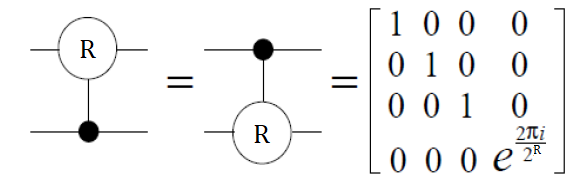
\includegraphics[width=1\textwidth]
{phaseshiftgate.png}
\captionsetup{format = hang}
\caption{Conditional phase shift gate critical for Fourier circuits.}
\label{fig:phaseshiftgate}
\end{figure}

At a high level, the design of the Fourier space circuit is similar to the classical based design, but with notable exceptions in the ADDER and ADDER MOD gates. The general strategy is to perform the resource-intensive addition tasks in Fourier space. In addition to requiring fewer auxiliary registers for the overall $U_f$ gate, the Fourier design allows a sharp reduction in the number of qubits needed in Register 1.

Before proceeding with a presentation of the modules used in the Fourier space circuit, we begin with some observations related to the QFT. We recall that a QFT on an integer state $|b\rangle$ on $n$ qubits performs the map
\begin{equation}
\label{eq:QFT}
|b\rangle \to \dfrac{1}{\sqrt{2^n}}  \mathlarger \sum_{z=0}^{2^n-1}\exp\left(\dfrac{2\pi i b z}{2^n}\right)|z\rangle.
\end{equation}

Let $|\phi(b)\rangle$ denote the QFT of $|b\rangle$. The right hand side of expression \eqref{eq:QFT} (i.e. $|\phi(b)\rangle$) can be factored as follows:
\begin{align}
|\phi(b)\rangle &= \dfrac{1}{\sqrt{2^n}} \mathlarger \sum_{z=0}^{2^n-1}\exp\left(\dfrac{2\pi i b z}{2^n}\right)|z\rangle \nonumber \\
&= \bigotimes_{z=0}^{n-1} \dfrac{1}{\sqrt{2}}\left(|0\rangle + \exp\left(\dfrac{2 \pi i b}{2^{z+1}} \right)|1\rangle\right) \nonumber \\
\label{eq:phib}
&= \bigotimes_{z=0}^{n-1} \dfrac{1}{\sqrt{2}}\left(|0\rangle + \exp\left(2\pi i (0.b_z\ldots b_0 \right)|1\rangle\right) \\
|\phi(b)\rangle &= \bigotimes_{z=0}^{n-1} |\phi_z(b)\rangle, \nonumber
\end{align} 
where $|\phi_z(b)\rangle = |0\rangle + \exp\left(2\pi i (0.b_z\ldots b_0 \right)|1\rangle$, and we have utilized binary fraction notation. We note that each $|\phi_z(b)\rangle$ term in equation \eqref{eq:phib} contains the bottom $z$ bits of the integer state $|b\rangle$. The goal with a quantum circuit that performs Fourier addition is to perform Fourier space rotations controlled by the bits of $a$, which is the value to be added to $b$. In particular, our goal is to implement a quantum plain ADDER circuit that outputs the following: 
\begin{equation}
\label{eq:fourieradder}
\bigotimes_{z=0}^{n-1} \dfrac{1}{\sqrt{2}}\left(|0\rangle + \exp\left(2\pi i (0.b_z\ldots b_0 + \mathbf{0.a_z \ldots a_0}\right)|1\rangle\right), 	
\end{equation}
where the value of expression \eqref{eq:fourieradder} is exactly equal to $|\phi(b+a)\rangle$. We can then extract and utilize the desired output information of $|b+a\rangle$ when necessary by applying inverse QFTs to exit Fourier space. As we will soon see, the Fourier space design requires several QFTs and inverse QFTs, which will contribute to the total number of gates needed to implement modular exponentiation. However, Draper and Beauregard's clever use of Fourier space results in a much smaller qubit requirement for the circuit overall. 




\subsection{Fourier ADDER and MOD ADDER}
The Fourier ADDER gate's goal is to take its input registers $|a\rangle|\phi(b)\rangle$ to the state $|a\rangle|\phi(b+a)\rangle$, which is accomplished by using a series of controlled phase shift gates. In figure \ref{fig:phiADDER}, the upper register contains the number $a$ on $n$ qubits, while the lower register contains $\phi(b)$, which is the QFT of a number $b$ on $n+1$ qubits. As was the case in Vedral's circuit, the answer register requires an extra qubit to handle any overflows from addition. The output value in the upper register remains unchanged from its input, while the answer register outputs the QFT of $b+a$.
\begin{figure}[!htbp]
\centering
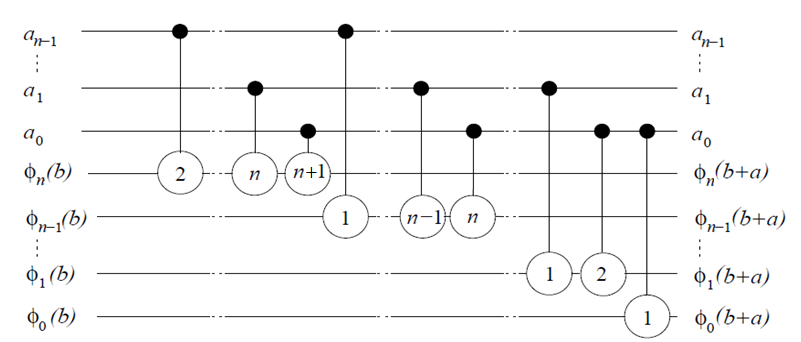
\includegraphics[width=1\textwidth]
{PHIadder.png}
\captionsetup{format = hang}
\caption{Draper's Fourier space ADDER gate. Adapted from \cite{Dra00}.}
\label{fig:phiADDER}
\end{figure}

To analyze the effect of the rotation gates, let us follow the action of the controlled phase shifts on the $z^\text{th}$ qubit in the lower register, i.e. on the single qubit representing $|\phi_z(b)\rangle$.
\begin{align*}
|\phi_z(b)\rangle &= \frac{1}{\sqrt{2}}\left(|0\rangle + \exp(2\pi i(0.b_z...b_0))|1\rangle\right) \\
&\to \frac{1}{\sqrt{2}}\left(|0\rangle + \exp(2\pi i(0.b_z...b_0 + 0.a_z))|1\rangle\right) && (a_z \text{ rotation}) \\
&\to \frac{1}{\sqrt{2}}\left(|0\rangle + \exp(2\pi i(0.b_z...b_0 + 0.a_z a_{z-1}))|1\rangle\right) && (a_{z-1} \text{ rotation})\\
& \vdots && \vdots\\
&\to \frac{1}{\sqrt{2}}\left(|0\rangle + \exp(2\pi i(0.b_z...b_0 + 0.a_z...a_0))|1\rangle\right) && (a_0 \text{ rotation}),\\
\end{align*}
where the final expression is corresponds to the $z^\text{th}$ term in expression \eqref{eq:fourieradder}. An immediately apparent benefit of Draper's Fourier space ADDER is the elimination of the $n$-qubit auxiliary carry register which was present in Vedral's design. As a result, the number of qubits needed to add two $n$ bit numbers is reduced from $3n+1$ to $2n+1$. However, there is still room for further improvement. 

Building on Draper's Fourier ADDER design, Beauregard proposed classically pre-computing the total phase shifts performed on each qubit \cite{Bea03}. This allows the for the elimination of the $n$ qubit register loaded with $a$, further reducing the number of qubits needed for Fourier space addition to $n+1$ (figure \ref{fig:phiADDERsmall}).
 \begin{figure}[!htbp]
\centering
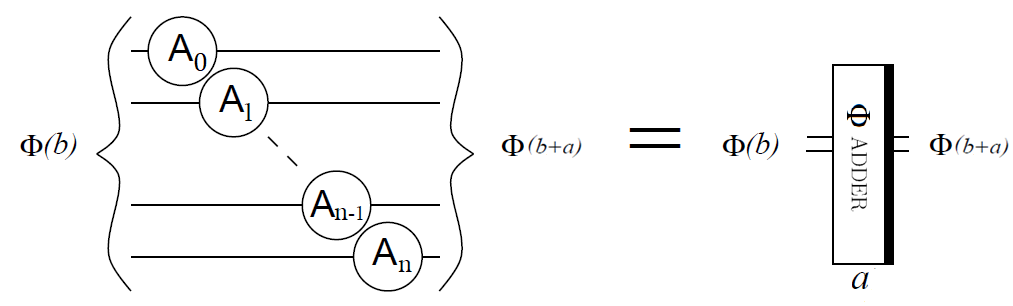
\includegraphics[width=0.85\textwidth]
{PHIadder_small.png}
\captionsetup{format = hang}
\caption{Beauregard's $\Phi$ADDER gate with precomputed rotation gates, $A_z$, acting on each qubit. Figure adapted from \cite{Bea03}.}
\label{fig:phiADDERsmall}
\end{figure}

The strategy for modular addition is similar to the one used in section \ref{sec:vedralADDERMOD}. However, since the $\Phi$ADDER gate has its inputs and outputs in Fourier space, the $\Phi$ADDER MOD gate requires QFT and $\text{QFT}^{-1}$ modules to extract and use the information of the MSB.
\pagebreak
 \begin{figure}[!htbp]
\centering
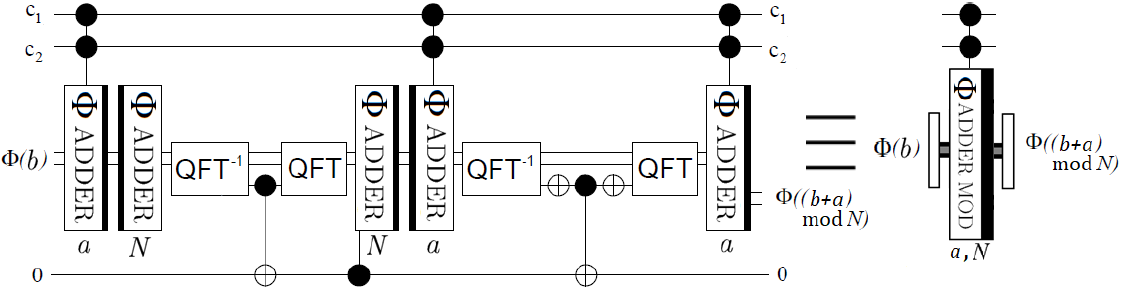
\includegraphics[width=1\textwidth]
{PHIADDERMOD2.png}
\captionsetup{format = hang}
\caption{Beauregard's $\Phi$ADDER MOD gate. The QFT and $\text{QFT}^{-1}$ modules allow for the use of the MSB of $b+a$ in a  role similar to the one performed by the MSB in figure \ref{fig:vedralADDERMOD}. Note the additional dependence on control qubits $c_1$ and $c_2$. If either control is in the $|0\rangle$ state, the output of the gate is $|\phi(b)\rangle$. Figure adapted from \cite{Bea03}.}
\label{fig:PHIADDERMOD}
\end{figure}

\subsection{Fourier Ctrl-MULT MOD gate}
Instead of including an extra register to perform the conditional loading of classical values as in figure \ref{fig:vedralCTRLMULTMOD}, Beauregard introduces a double control dependence to the $\Phi$ADDER MOD gate (figure \ref{fig:PHIADDERMOD}). The first control, $c_1$, corresponds to the qubit in Register 1. The second control, $c_2$,  corresponds to a qubit in the binary representation of a number $\gamma$, which will be the output from the preceding $\Phi$Ctrl-MULT MOD gate. This $\gamma$ is similar to the one in figure \ref{fig:vedralCTRLMULTMOD}). 
\begin{figure}[!htbp]
\centering
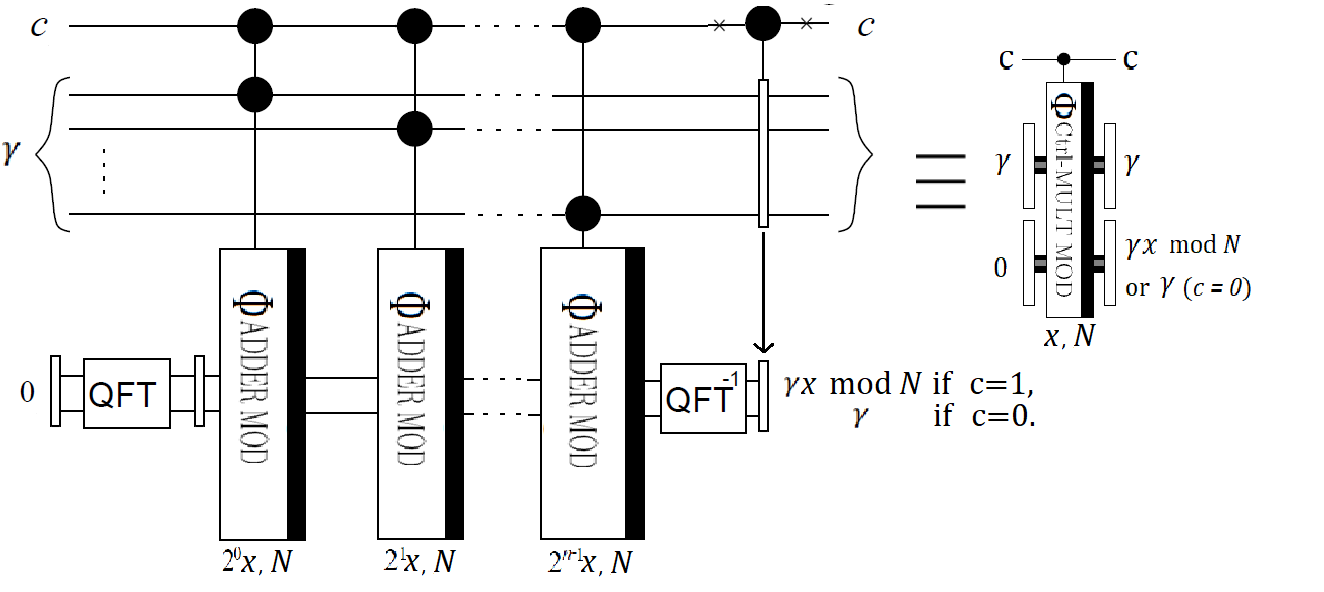
\includegraphics[width=1\textwidth]
{PHICTRLMULTMOD.png}
\captionsetup{format = hang}
\caption{Beauregard's $\Phi$Ctrl-MULT MOD gate. Note the similarity to Vedral's Ctrl-MULT MOD (figure \ref{fig:vedralCTRLMULTMOD}), but with additional QFT and $\text{QFT}^{-1}$ modules.  
Figure adapted from \cite{Bea03}.}
\label{fig:PHICTRLMULTMOD}
\end{figure}

We note that the $\Phi$Ctrl-MULT MOD circuit is very similar to Vedral's classical-based Ctrl-MULT MOD circuit. One notable difference is the presence of QFT and $\text{QFT}^{-1}$ modules to allow the addition modules to operate in Fourier space. A second difference is that the controlling qubit is not related to $|k_j\rangle$ (the $j^{\text{th}}$ qubit of the  state $|k\rangle$ in Register 1). Instead, all $\Phi$Ctrl-MULT MOD modules in the final circuit are controlled by a single qubit.

As Beauregard shows in \cite{Bea03}, if the lower input register of the $\Phi$Ctrl-MULT MOD gate is not in the $|0\rangle$ state, the output will be $|(b+\gamma x) \text{ mod }N\rangle$ (for $|c\rangle=|1\rangle$). However, as we will see in the following section, the lower register's input will always be $|0\rangle$ due to the way the gates are networked in the final circuit with swaps and modular inverses. Thus, for our purposes, it suffices to only consider the case when the lower register is in the $|0\rangle$ state, as is the case with Vedral's Ctrl-MULT MOD circuit in figure \ref{fig:vedralCTRLMULTMOD}. 


\subsection{The one controlling qubit trick}
\label{sec:1ctrltrick}
Beauregard's One-Ctrl qubit trick \cite{Bea03} involves some small deviations from the steps of Shor's period finding algorithm outlined in section \ref{sec:ShorsDescription}. For instance, steps 3-5 are performed non-sequentially. Most significantly, the One-Ctrl qubit trick allows us to bypass step 2, which involves the creation of a superposition state on the $t\geq 2n$ qubits of Register 1. 
\begin{figure}[!htbp]
\centering
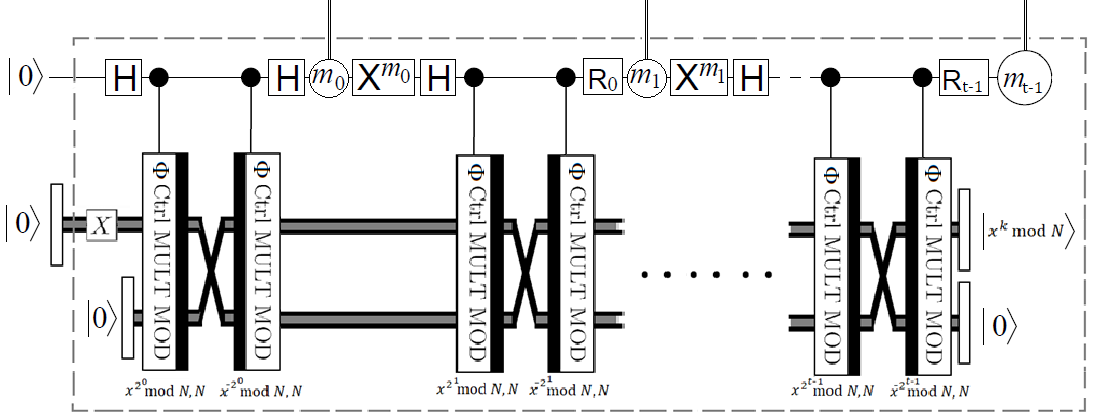
\includegraphics[width=1\textwidth]
{PHIEXPMOD.png}
\captionsetup{format = hang}
\caption{A modified version of Beauregard's circuit with the One-Ctrl qubit trick. The first measurement result, $m_0$, corresponds to the least significant bit of the desired output of Shor's algorithm.}
\label{fig:PHIEXPMOD}
\end{figure}

Measurements on the controlling qubit dictate the transformations to apply after each pair of $\Phi$Ctrl-MULT MOD gates. The conditional X gates ensure the re-purposed qubit is ``reset'' to the $|0\rangle$ state after each measurement. The $R_k$ phase gates are given by 
\begin{equation*}
R_k = \left( \begin{matrix} 1&0\\ 0&e^{i \theta_k} \end{matrix} \right), \qquad \text{  where  } \theta_k = \pi \sum_{j=0}^{k-1} 2^{k-j}m_j.
\end{equation*}
The sum in the calculation of $\theta_k$ runs over the $k$ previous measurements and $m_j \in \{0,1\}$ denotes the $j^\text{th}$ measurement result. The effect is to simulate a QFT and subsequent measurement of Register 1 as in figure \ref{fig:shorscircuit}. I.e. the measurement readout (step 5) occurs bit-by-bit alongside the application of the modular exponentiation function (step 3) and the Quantum Fourier Transform (step 4).  Thus, an implementation of Beauregard’s circuit with the One-Ctrl qubit trick (figure 15) would perform the same function as the high-level Shor’s algorithm circuit shown in figure 2.

\section{Qubit requirement analysis}
We now present some brief analyses of the qubit requirements for Vedral's classical-based circuit and Beauregard's Fourier space circuit. These analyses are also present in the respective authors' original papers (\cite{VBE95}, \cite{Bea03}), but are included here for completeness. 

Before accounting for auxiliary registers, Vedral's classical-based circuit requires at least $2n$ qubits in Register 1 to hold the superposition of integer states $|k\rangle$, and $n$ qubits in Register 2 to hold the output $|x^k \text{ mod } N\rangle$. The ADDER gates (figure \ref{fig:vedralADDER}) require an extra $(n-1)$-qubit register to facilitate carries, and one qubit to handle addition overflow. The ADDER MOD gates (figure \ref{fig:vedralADDERMOD}) require an $n$-qubit register to store $N$, and one extra auxiliary control qubit. The Ctrl-MULT MOD gates (figure \ref{fig:vedralCTRLMULTMOD}) also require another $n$-qubit register to conditionally load the classically computed $2^m x^{2^j} \text{ mod }N$ values. Finally, the construction of the modular exponentiation gate (figure \ref{fig:vedralexpmod}) requires an extra $n$-qubit register to facilitate resets via modular inverses. In total, Vedral's design requires $7n+1$ qubits to factor an $n$-bit number, with $4n+1$ qubits coming from the auxiliary registers. 

With Beauregard's One-Ctrl qubit trick, the size of Register 1 is effectively reduced to a single qubit. As in the classical ADDER gates, the $\Phi$ADDER gates (figure \ref{fig:phiADDERsmall}) require an additional qubit to prevent overflow. However, Fourier space addition removes the need for an extra $n$-qubit auxiliary register. The $\Phi$ADDER MOD gates (figure \ref{fig:PHIADDERMOD}) also require a single additional control qubit, but do not need an additional register to store $N$. Finally, the $\Phi$Ctrl-MULT MOD gates (figure \ref{fig:PHICTRLMULTMOD}) require an additional $n$-qubit register to facilitate swaps and resets. In total Beauregard's Fourier space architecture requires $2n+3$ qubits to factor an $n$-bit number, with $n+2$ qubits coming from the auxiliary registers. 

Although classical-based circuits require more qubits, they have several advantages over Fourier space circuits. For instance, the Fourier space ADDER circuit requires several computations to create problem-specific phase shift gates (figure \ref{fig:phiADDERsmall}). In addition, classical-based circuits are more easily simulated, whereas debugging Fourier space circuits is more difficult. Although a variety of different circuit implementations exist, each faces its own challenges with testability and space/time trade-offs. A familiarity with the two main architectures is the first step to tackling these challenges. 

\section*{Acknowledgements}
The author wishes to thank Prof. Anne Broadbent for providing the opportunity to research this topic, along with generous funding and valuable advice throughout the duration of the project. In addition, the author wishes to thank Profs. Daniel Fiorilli and Anne Broadbent for supervising the project and furthering the author's interest in mathematics.







\bibliographystyle{alphaarxiv.bst} \bibliography{full.bib,quantum.bib} 

\pagebreak

\appendix
\section{Appendix: Detailed example}
We provide a detailed example of obtaining the factors of an integer, $N = 21$, using Shor's factoring algorithm. Using prior knowledge of the period, $r$, of a chosen $x \text{ }(\text{mod } 21$), we attempt a classical explanation of the workings of Shor's algorithm. In particular, we show how to obtain an analytic expression for the probability spectrum of measuring some particular integer value in Register 1, assuming prior knowledge of $r$. In addition to its pedagogical value, this analytic expression can be used to verify the result of a real experiment.

For simplicity, we will use a quantum circuit similar to Vedral's design (figure \ref{fig:levelscheme}). Additionally, we use $t=7$ qubits in both Register 1 and Register 2. Ideally, we would use $n = \ceil*{\log_2(N)}$ in Register 2, and $t\geq 2n$ qubits in Register 1 for good precision. As described in section \ref{sec:ShorsDescription}, we begin the quantum part of Shor's period finding algorithm by initializing our quantum registers to the zero state. Our machine begins in the state
\begin{equation*}
|0\rangle|0\rangle = |0000000_2\rangle|0000000_2\rangle.
\end{equation*}
Follow the initialization step, we apply Hadamard gates to each qubit in Register 1 to create a superposition state. More formally, we perform the following operation on our initial state:
\begin{equation*}
|0\rangle|0\rangle \xrightarrow{H^{\otimes 7}} \dfrac{1}{\sqrt{2^7}} \sum_{k=0}^{2^7-1}|k\rangle|0\rangle,
\end{equation*}
where the right hand side of the above expression is equal to 
\begin{align*}
& \dfrac{1}{\sqrt{2^7}}\left(|0\rangle + |1\rangle + ... + |127\rangle\right) |0\rangle \\
=&  \dfrac{1}{\sqrt{2^7}} \left(|0000000_2\rangle + |0000001_2\rangle + ... + |1111111_2\rangle \right) |0000000_2\rangle.
\end{align*}
Once we have set up the superposition on Register 1, we apply the $U_f$ function, which introduces entanglement between the Register 1 and Register 2. For simplicity, suppose $U_f$ is implemented using Vedral's circuit discussed in section \ref{sec:VedralSec}. For a chosen $x = 5$, the $U_f$ module performs the following map:
\begin{equation*}
\dfrac{1}{\sqrt{2^7}} \sum_{k=0}^{2^7-1}|k\rangle|0\rangle \xrightarrow{U_f} \dfrac{1}{\sqrt{2^7}} \sum_{k=0}^{2^7-1}|k\rangle|5^k \text{ mod } 21\rangle,
\end{equation*}
where the right hand side of above equation is equal to
\begin{align*}
\dfrac{1}{\sqrt{2^7}} (&|0\rangle |5^0 \text{ mod } 21\rangle + |1\rangle |5^1 \text{ mod } 21\rangle + \ldots +\\
&|126\rangle |5^{126} \text{ mod } 21\rangle + |127\rangle|5^{127} \text{ mod } 21\rangle) \\
= \dfrac{1}{\sqrt{2^7}} (&|0\rangle |1\rangle + |1\rangle |5\rangle + |2\rangle |4\rangle + |3\rangle |20\rangle + |4\rangle |16\rangle + |5\rangle|17\rangle + \\
& |6\rangle |1\rangle + |7\rangle|5\rangle + |8\rangle |4\rangle  + |9\rangle |20\rangle + |10\rangle |16\rangle + |11\rangle |17\rangle + ... +\\
& |123\rangle|4\rangle + |124\rangle|20\rangle + |125\rangle|17\rangle + |126\rangle|1\rangle + |127\rangle|5\rangle).
\end{align*}
From the above expression, we can clearly see $r=6$, i.e. the period of $5 \text{ mod } 21$ is 6. However, this information is hidden from the user of the quantum computer. In order to extract the information of the period into something measurable, we must perform a Quantum Fourier Transform. Before we continue with the example, we briefly discuss the mechanics of a QFT on Register 1. For additional details, readers can refer to \cite{Dra00}, which discusses a quantum circuit implementation of the QFT in detail.

As discussed in section \ref{sec:ShorsDescription}, a QFT puts the machine in the state	
\begin{equation}
\label{eq:QFTstate}
\dfrac{1}{2^t}\sum_{k=0}^{2^t-1}\sum_{y=0}^{2^t-1}\exp\left( \dfrac{2\pi i ky}{2^t} \right)|y\rangle |x^k \text{ mod } N\rangle. 
\end{equation}
Recall that $x^k \text{ mod }$ is periodic with period $r$, so that we can write $x^k \text{ mod } N = x^{\widetilde{k} + lr} \text{ mod } N$, where $0\leq \widetilde{k} < r$ is the residue of $k \text{ modulo } r$. Let $L$ be the maximum possible value of $l$ ($L$ is dependent on $t$ and $\widetilde{k}$). We can then rewrite expression \eqref{eq:QFTstate} as follows: 
\begin{equation}
\label{eq:QFTstatewithperiod}
\dfrac{1}{2^t}\sum_{\widetilde{k} = 0}^{r-1}\sum_{\widetilde{y} = 0}^{2^t-1}\sum_{l=0}^{L} \exp\left(\dfrac{2\pi i (\widetilde{k}+lr)\widetilde{y}}{2^t}\right)|\widetilde{y}\rangle|x^{\widetilde{k}} \text{ mod } N,
\end{equation}
where each $\widetilde{y}$ is the quantity associated with the corresponding $\widetilde{k}$. From expression \eqref{eq:QFTstatewithperiod}, we can observe that the information of the period, $r$, has been encoded within the amplitudes after applying the QFT. When we perform the measurement of Register 1, these amplitudes are related to the probability of observing a particular state $|\widetilde{y}\rangle|x^{\widetilde{k}} \text{ mod }N\rangle$ as follows:
\begin{equation}
\label{eq:prob}
Pr(\widetilde{y},\widetilde{k}, r) = \left(\dfrac{1}{2^t}\right)^2\left|\sum_{l=0}^{L} \exp\left(\dfrac{2\pi i l r \widetilde{y}}{2^t}\right)  \right|^2.
\end{equation}

Continuing with the values in our example, we have the state of our machine after the QFT given by
\begin{equation*}
\dfrac{1}{2^7}\sum_{k=0}^{2^7-1}\sum_{y=0}^{2^7-1}\exp\left( \dfrac{2\pi i ky}{2^7} \right)|y\rangle |5^k \text{ mod } 21\rangle. 
\end{equation*}
As we showed in expression \eqref{eq:QFTstatewithperiod}, the above expression encodes information about the period $r$, and is equivalent to 
\begin{equation*}
\dfrac{1}{2^7}\sum_{\widetilde{k} = 0}^{6-1}\sum_{\widetilde{y} = 0}^{2^7-1}\sum_{l=0}^{L} \exp\left(\dfrac{2\pi i (\widetilde{k}+6l)\widetilde{y}}{2^7}\right)|\widetilde{y}\rangle|5^{\widetilde{k}} \text{ mod } N \rangle.
\end{equation*}

In equation \eqref{eq:prob}, we discussed the probability of observing some particular 
$|\widetilde{y}\rangle|5^{\widetilde{k}} \text{ mod }21\rangle$, such as $|\widetilde{y}\rangle|20\rangle (\implies \widetilde{k} = 4, \text{ since } 5^4 \text{ mod } 21 = 20)$. Suppose we wish to find an analytic expression for the probability spectrum as a function of only $\widetilde{y}$ (and hidden $r$). We can obtain such an analytic expression by summing over all residues $\widetilde{k}$ of $k$ modulo $r$. Table \ref{table:table1} shows the appropriate values of $L$ to use in the summations. 

\begin{table}[!htbp]
\centering
\begin{tabular}{|c|c|c|c|c|c|c|}
\hline
$\widetilde{k}$ & 0 & 1 & 2 & 3 & 4 & 5 \\ \hline
$5^{\widetilde{k}} \text{ mod } 21$ & 1 & 5 & 4 & 20 & 16 & 17 \\ \hline
$L=\text{max}(l)$ & 21 & 21 & 20 & 20 & 20 & 20 \\
\hline
\end{tabular}
\captionsetup{format=hang}
\caption{Table of classically computed information. The period of $5 \text{ mod }21$ is 6, so there are 6 residue classes $\widetilde{k}$. The maximum value of $l$ is dependent on the number of times $r$ divides $2^t-1$, but $L$ will be approximately the same for all residue classes.}
\label{table:table1}
\end{table}
The analytic expression for the probability spectrum is given by 
\begin{equation}
\label{eq:explicitformula}
Pr(\widetilde{y}) = \left(\dfrac{1}{2^t}\right)^2\left(2\left|\sum_{l=0}^{21}\exp\left(\dfrac{2\pi il6\widetilde{y}}{2^7}\right)  \right|^2  + 4\left|\sum_{l=0}^{20}\exp\left(\dfrac{2\pi il6\widetilde{y}}{2^7}\right) \right|^2 \right).
\end{equation}
Although explicit formulae such as the one shown in equation \eqref{eq:explicitformula} are unobtainable without prior knowledge of $r$, they can be useful for pedagogical reasons, or to verify an experimentally obtained probability distribution.
\begin{figure}[!htbp]
\centering
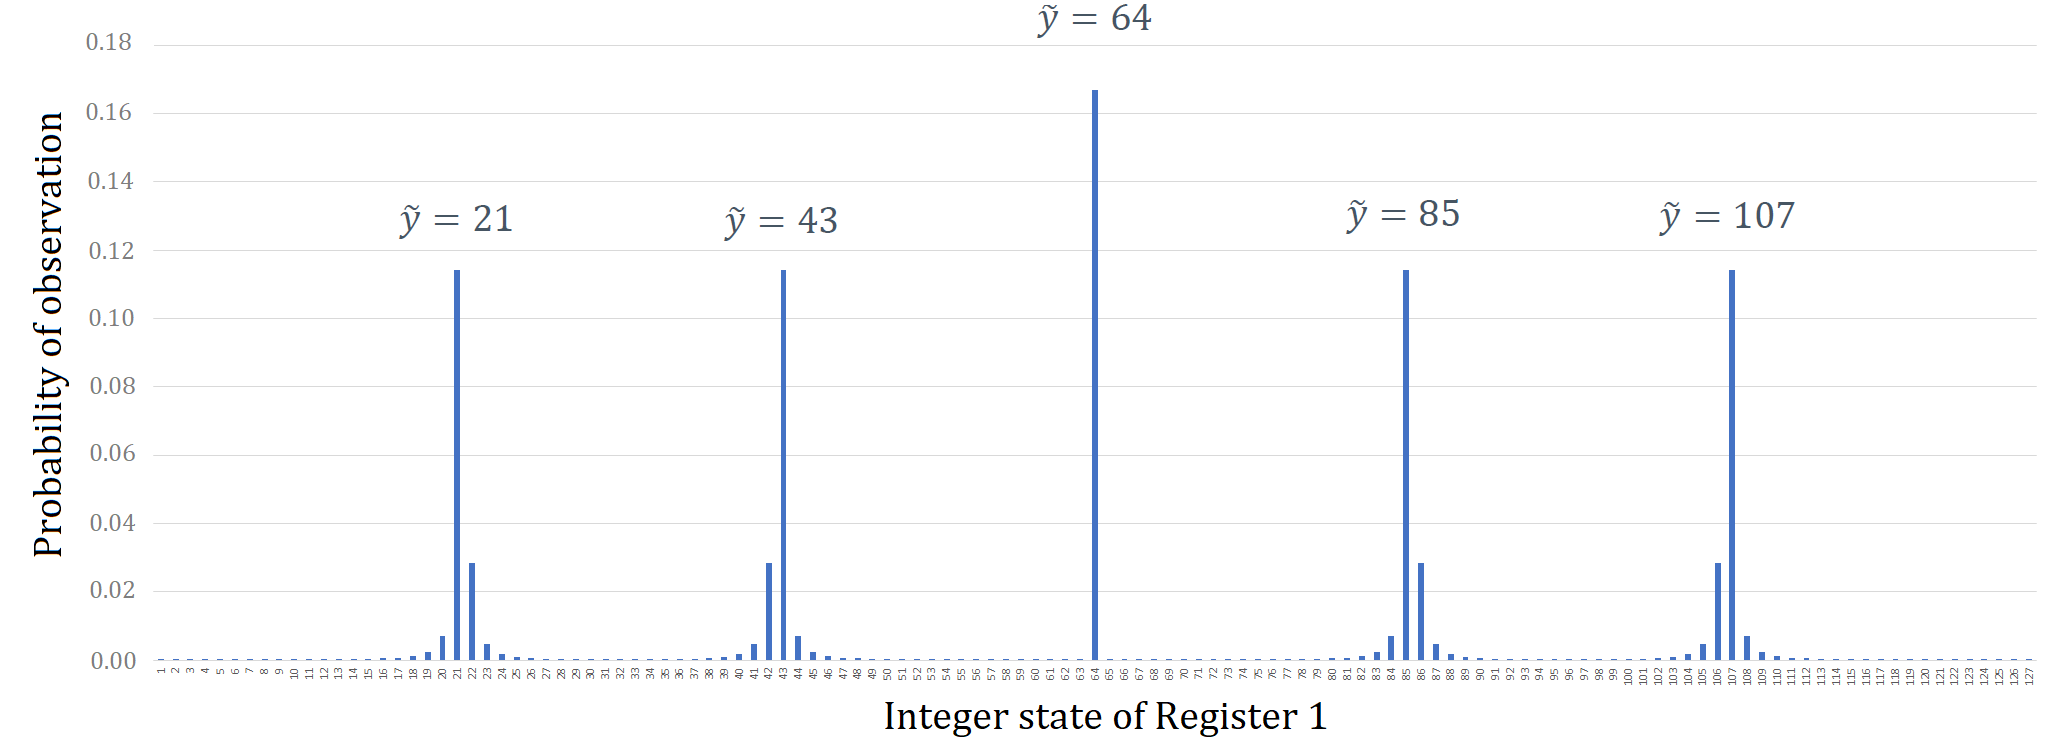
\includegraphics[width=1\textwidth]
{p_spectrum.png}
\captionsetup{format = hang}
\caption{The probability spectrum for $x=5$ and $N=21$ as a function of the integer state of Register 1. We have omitted the probability peak (probability of around 0.16) at $\widetilde{y} = 0$, as this result is not usable for factoring.}
\label{fig:probspectrum}
\end{figure}

By observing equation \eqref{eq:prob}, we can see that the probabilities for each residue $\widetilde{k}$ peak at a value of $\left(\dfrac{L+1}{2^t}\right)^2$ when $\dfrac{r\widetilde{y}}{2^t} \in \mathbb{Z}$. Thus, the locations of the probability peaks (as a function of $\widetilde{y}$) contain the information of $r$ as an integer multiple of $\dfrac{2^t}{\widetilde{y}}$. Since $t$ is set by the user and each $\widetilde{y}$ is known from measurement, we can perform multiple measurements and extract $r$ using efficient classical techniques. 

Following the measurement of Register 1, we perform classical post-processing of the measurement result. In particular, we use the method of continued fractions to extract the period from the measurement result. Our goal is to find $\dfrac{\beta}{r}$ satisfying $\left|\dfrac{\widetilde{y}}{2^t} - \dfrac{\beta}{r}\right|\leq\dfrac{1}{2^{t+1}}$, with $\beta \in \mathbb{Z}$. Recall that the simple continued fraction expansion of a real number $R$ is of the form
\begin{equation}
R = a_0 + \dfrac{1}{a_1+\dfrac{1}{a_2+\dfrac{1}{...}}}.
\end{equation}
Also recall that the \textit{convergents} of the continued fraction are rational approximations of $R$. Shor's idea is to use the convergents of $\dfrac{\widetilde{y}}{2^t}$ to obtain $\dfrac{\beta}{r}$ in lowest terms, such that $\left|\dfrac{\widetilde{y}}{2^t} - \dfrac{\beta}{r}\right|\leq\dfrac{1}{2^{t+1}}$ is satisfied. An intuitive interpretation would be to make $\dfrac{\widetilde{y}}{2^t} \approx \dfrac{\beta}{r}$ up to some small error outside the possible resolution of computer's $t$ qubits.  

The first two convergents of a real number $R$ are given by 
\begin{equation*}
\dfrac{\beta_0}{r_0} = \dfrac{a_0}{1}, \qquad \dfrac{\beta_1}{r_1} = \dfrac{a_0a_1+1}{a_1}.
\end{equation*}
The $j^\text{th}$ convergent $\dfrac{\beta_j}{r_j}$ is given by the following recursive expression:
\begin{equation*}
\dfrac{\beta_j}{r_j} = \dfrac{a_n\beta_{n-1} + \beta_{n-2}}{a_nr_{n-1}+r_{n-2}}.
\end{equation*}
Suppose we measure $\widetilde{y} = 107$ in Register 1. Our goal is to find $\dfrac{\beta}{r}$ such that $\left|\dfrac{107}{128}-\dfrac{\beta}{r}\right| \leq \dfrac{1}{256}$. The relevant continued fraction is
\begin{equation*}
\dfrac{107}{128} = 0 + \dfrac{1}{1+\dfrac{1}{5+\dfrac{1}{10+\dfrac{1}{2}}}}.
\end{equation*}
The first three convergents are given by
\begin{equation*}
\dfrac{\beta_0}{r_0} = \dfrac{0}{1}, \qquad \dfrac{\beta_1}{r_1} = \dfrac{1\cdot 0 + 1}{1}, \qquad \dfrac{\beta_2}{r_2} = \dfrac{5\cdot 1 + 0}{5\cdot 1 + 1} = \dfrac{5}{6}.
\end{equation*}
Reading off the value from $r_2$, we see that the period is $6$. All that remains before the final step of computing greatest common divisors is to check that $x^{r/2} \not \equiv \pm 1 \text{ mod }N$. However, we find that $5^3 \equiv -1 \text{ mod } 21$. As this will give us a trivial factor of $N$, we must choose a new $x$ and repeat the entire period finding process. Suppose we next choose $x=11$. After setting up the circuit and performing measurements, we again find $r=6$ for $x=11$ and $N=21$. We conclude by computing the factors of $N$ as follows:
\begin{align*}
p &= \gcd(x^{r/2} - 1, N) \qquad \to \qquad  p = \gcd(11^{6/2}-1, 21) \\
q &= \gcd(x^{r/2} + 1, N) \qquad \to \qquad q = \gcd(11^{6/2}+1, 21).
\end{align*}
Finally, we find that $p = 7$ and $q=3$.











\end{document}

